\chapter{Hardware setup}
The hardware must be physically attached in order to reach the goal of a closed loop controller for a handshake. From early approaches as \cite{knoop2017handshakiness}, an estimation of the human palm has been used.  The sensorized palm is an approximation of the human palm, simple 3D-printed whose shape and dimensions similar to a human hand palm, composed of two shells connected by a load cell.
The required approximation consists in assuming that after the first contact point is reached, increasing the reference position is not modifying the shape of the sensorized palm accordingly, human hand palm is modelled as a rigid body. %The interaction between the human hand and the robot hand is therefore assumed to be interaction between rigid bodies.
The figure \ref{fig:sensorsONhand} shows the position in which the sensors $1$ and $2$ are placed according studies in \cite{knoop2017handshakiness}. \\ \\
%, the sensor n. 4 is placed in order to increase the weight of human-thumb force applied during the grasp.\\ \\

\begin{figure}[h]
  \centering
  \begin{minipage}[b]{0.45\textwidth}
    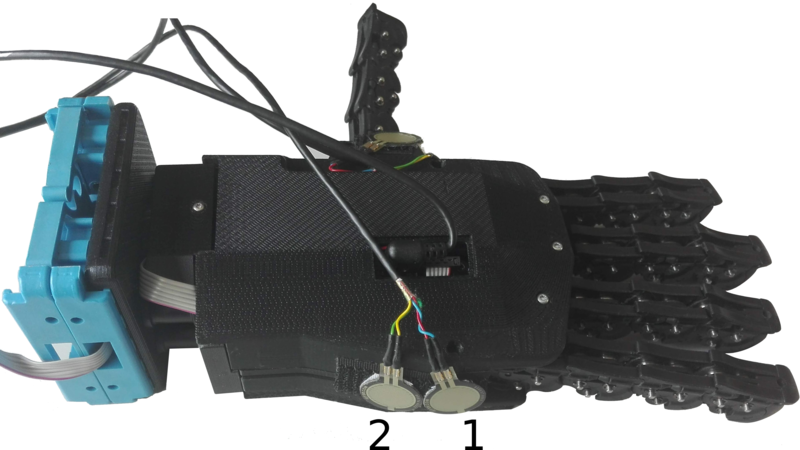
\includegraphics[width=\textwidth]{Figure/qbhand2-small.png}
  \end{minipage}
  \hfill
  \begin{minipage}[b]{0.45\textwidth}
    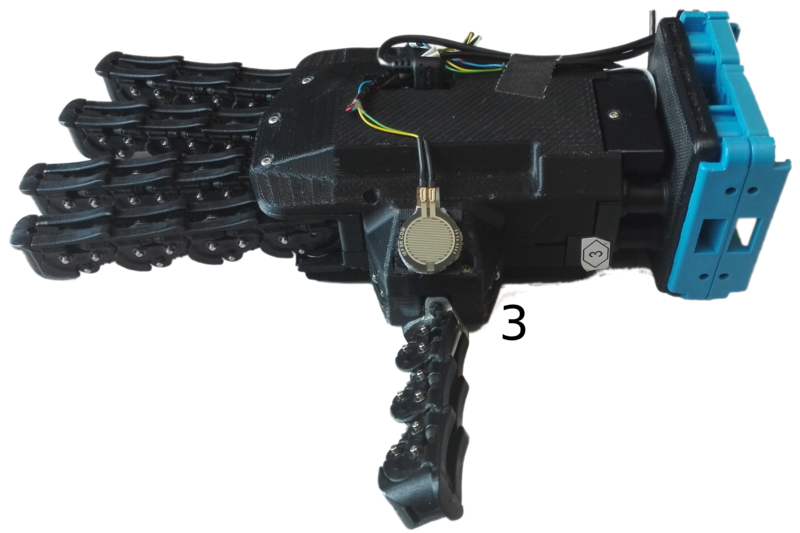
\includegraphics[width=\textwidth]{Figure/qbhand1-small.png}
  \end{minipage}
  \label{fig:sensorsONhand}
  \caption{Pisa/IIT SoftHand with FSR sensors for handshake}
\end{figure}

Histogram from \cite{knoop2017handshakiness} is used as a guide for where to place the sensors, using the notation $F_{fsr,i}$, with $i = 1\cdots 3$, for the measure of the generic sensor. 
%
Sensors $1-3$ in Fig.~\ref{fig:sensorsONhand}, are used as triggers to identify the contact with the human hand, and $1$ and $2$ are used for estimating robot force as they were found to be robust towards small variations in the grasp. 


\section{The Pisa/IIT SoftHand}\label{sec:softhand}
The Pisa/IIT SoftHand is a simple, robust and effective hand designed for grasping and soft manipulation presented in \cite{catalano2014adaptive}. 
%A tick range is provided with the device in order to set a range of possible closure positions, more formally, let's define $q \in \mathbb{N}$ as the closure position of the hand such that $max(q) = 19000$ (Pisa/IIT SoftHand fully closed) and $min(q)=0$ (Pisa/IIT SoftHand fully open). 
The hardware is provided with a controller developed by the same group which implements a proportional controller, generically sketched in Fig. \ref{Fig:Pr}, on the motor position. This enables the researchers to control the Pisa/IIT SoftHand with a reference position, without dealing with the current control of the motor. \\
%
\begin{figure}[h]
\centering
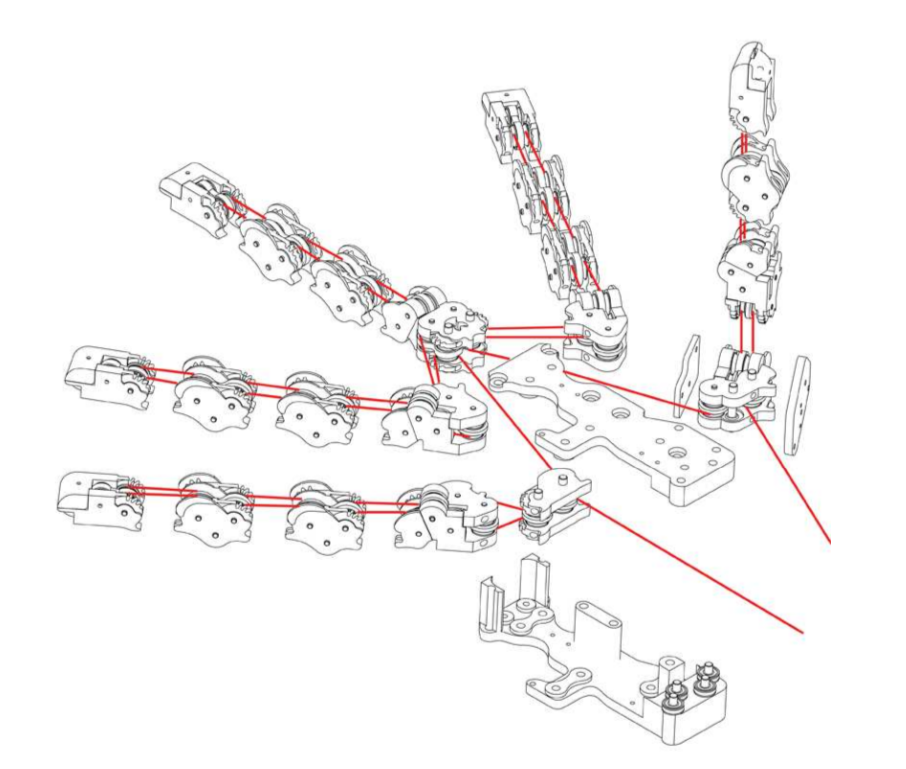
\includegraphics[width=0.6\textwidth]{Figure/softhand.png}
\caption{Exploited view of the modules of Pisa/IIT SoftHand}
\label{Fig:Softhand}
\end{figure}
%
The proportional coefficient can be set up as preferred since its encoded in ROS as a \textit{rosparam}, this parameter is thought to range between 0 and 1.0. Setting the parameter to 1.0 is minimizing the error value $e(t)$  between the setpoint $r(t)$ and the output $y(t)$.
The successful idea in the design of Pisa/IIT SoftHand can be found in the flexibility of the joints and the wide range of usage.
%The reference position $r(t)$ has no 1:1 correspondence with the single physical position of each finger. 
Having a single motor to control makes the robotic hand really easy to control but introduce uncertainty on the position of each finger. 
A tendon is running through all the fingers and is pulled by the internal dc motor, therefore a useful available information is the overall tick-position of the Pisa/IIT SoftHand. Constraints on the closure position $q$ are defined as follows:

\begin{equation}
q \in \mathbb{N} : \left\{\begin{matrix}
max(q) = 19000 & $ (robot hand fully close) $ \\ 
min(q) = 0 & $ (robot hand fully open)$
\end{matrix}\right.
\label{eq:qlimits}
\end{equation}

The device has an internal value returning to the system the real tick position $q_{output}$, this value is compared with the referenced one in the controller $q_{ref}$. The real tick position is a value that must be calibrated manually using administrative tools provided by the manufacturers. 
The calibration is manual which means that the robot hand is manipulated to be into a fully open position and the program save that position as the zero tick position.
%The controller used $C(s)$ is a simple constant controller with value ranges from 0 to 1. 

\begin{figure}[h]
\centering
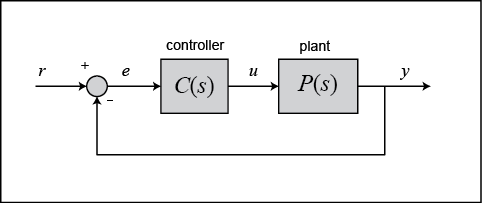
\includegraphics[width=0.5\textwidth]{Figure/feedbackP.png}
\caption{Block Diagram Proportional controller in a feedback loop}
\label{Fig:Pr}
\end{figure}


\section{The Sensors}
The core of a closed loop controller for human-robot handshake is to control the robot force $F_{r}$ given the human force $F_{h}$. FSR sensors are used for measuring the human force but mathematical tools are used to estimate the robot force from its pose. 

\begin{wrapfigure}{R}{0.3\textwidth}
\centering
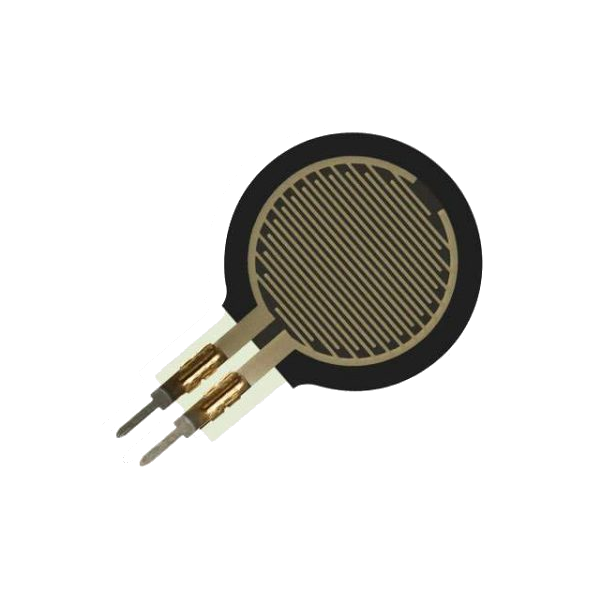
\includegraphics[width=0.25\textwidth]{Figure/fsrsingle1.png}
\caption{FSR 13mm}
\label{Fig:FSRsingle}
\end{wrapfigure}

The Force Sensitive Resistors used are placed on the robot hand in a strategical position for two main reasons:
\begin{itemize}
\item the study in \cite{knoop2017handshakiness} shows that the grasping force on the approximation of the human palm, is highly involving the considered hand area.
\item the task is to measure the human grasping force $F_{h}$, and this position enables a decouple from the robot grasping force $F_{r}$.
\end{itemize}
%The sensors used in this work are Force Sensitive Resistors Fig. \ref{Fig:FSRsingle} measuring the force applied from the human to the robot hand, in order to decouple this force from the one applied from the robot to the human, \cite{knoop2017handshakiness} has been used and the physical position of the FSRs has been setted up accordingly.

The FSR sensors are devices that allow to measure static and/or dynamic forces applied on the sensing area, through the variation of its electric resistance. The main advantage of these devices is the low cost per-unit, little space required for installation (thickness under 1.25mm) and the force sensitivity range up to 100N.\\
As robust polymer thick film devices, the FSRs, exhibit a decrease in electric resistance with increase in force applied to the surface. By theory is considered that when a force is applied the resistance changes approximately linear in a logarithmic plot \cite{fsrdatasheet}.
A simple force to voltage conversion is physically implemented as suggested the manifacturer, in fig. \ref{Fig:FSRcircuit} is shown a snippet of the above cited data sheet. For this work \textit{RM} is fixed to $3.3 k \Omega $. \\
\begin{figure}[ht]
\centering
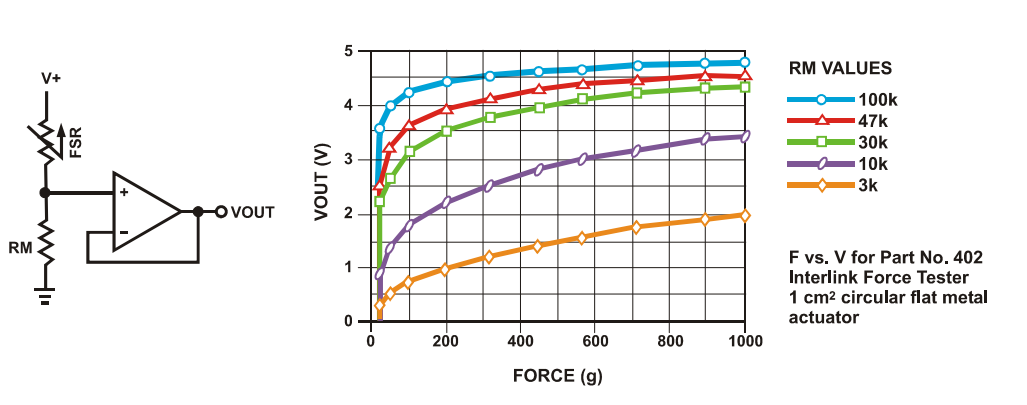
\includegraphics[width=0.8\textwidth]{Figure/fsr.png}
\caption{FSR Datasheet snippet}
\label{Fig:FSRcircuit}
\end{figure}
These mentioned sensors are the more natural choice for handshake experiments since their thickness keeps the size of the robot hand reasonable for the task.
% 
Ideally using more sensors allow to get more relevant data but the surface available on the Pisa/IIT SoftHand is limited. The choice in the number of FSR sensors comes from the trade off between using lots of FSR sensors but with a smaller area and using a smaller amount of sensors but with higher area. The first configuration does not ensure the contact among experiments with different participants and the second configuration leads to physical bending of the sensors and influences the consistency of the readings.

 %A calibration method must be used in order to have robust results.

\subsection{Calibration of FSRs}\label{subsec:calibFSR}
The calibration procedure of a sensor is a really important task, since it allow to compare experiments and to provide consistent results. 
The first voltage-to-force relation for the FSRs comes from a manufacturer sketch which is returning force proportionally with standard of gram-force. This first approach is considered not consistent so an ad-hoc calibration experiment is required.
As shown in \cite{calibFSR}, load cells can be used as 'ground truth' to calibrate force sensitive resistors.% to provide informations in Newtons. 
Using a \textit{sensorized palm} developed in \cite{knoop2017handshakiness}, sketched in Fig. \ref{fig:dummi} which embeds a load cell and placing the FSR sensors accordingly with the position of the sensors $1$ and $2$ on the Pisa/IIT SoftHand \ref{fig:sensorsONhand}; values from FSRs and the load cell are compared.\\
Mathematical regression tools have been used in order to find a model that explain the values from the sensors compared to the force of the load cell.
Although an exact calibration of FSR sensors is not the target of this work, a model has been fitted to the data in the force-range of interest of this work.
%The number of FSR sensors involved in the calibration experiment is two, instead the amount of FSR sensors chosen for the human-robot handshake is four. 
The configuration for the calibration experiment, with the \textit{sensorized palm} and two FRS sensors is shown in Fig. \ref{fig:dummifsr}. 
%The position of the FSR sensors has been chosen accordingly to the position of the FSR sensors N.1 and N.2 on the Device \ref{fig:sensorsONhand}.
%In order not to add complexity to this task, is assumed that using two FSR are sufficient to fit a model to the FSR sensors involved in the handshake environment.
The experiment consist in apply a grasp to the device including not exclusively, the FSR sensors in the grasp. Six calibration experiments were performed, with three different subjects. In each test, the subject was asked to repeatedly grasp and release the sensorized palm, and FSRs and load cell values were recorded. A cubic polynomial is fitted to the data, as shown in Fig.~\ref{Fig:FSRcalibratedModel}. This allows to estimate $F_{h}$. Although there is some error in the fit, it is observed that for a given handshake grasp between a participant and the robot the estimate of $F_{h}$ is monotonic and with relatively low variation---the main source of variation is variations in the human grasp configuration.%, obtaining the relation in eq.~\eqref{eq:fh}. Measured data and results of fitting process are summarized in Fig.~\ref{fig::fsrdummypalm}. 
% In post processing a model is fitted to the data and eventually allow the FSR to correcly estimate the grasping force.

\begin{figure}[h]
  \centering
  \begin{minipage}[b]{0.4\textwidth}
    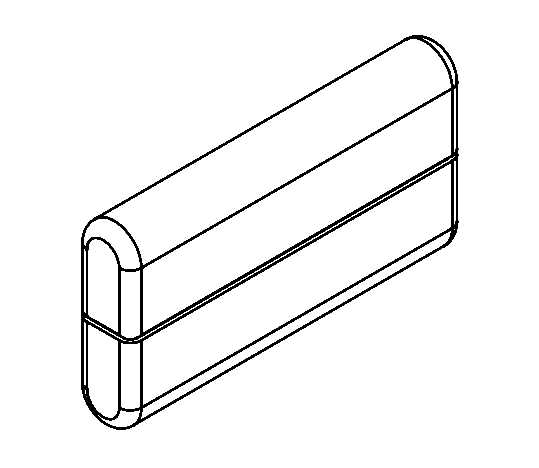
\includegraphics[width=\textwidth]{Figure/dummipalm.png}
    \caption{Sensorized palm}
  \label{fig:dummi}
  \end{minipage}
  \hfill
  \begin{minipage}[b]{0.4\textwidth}
    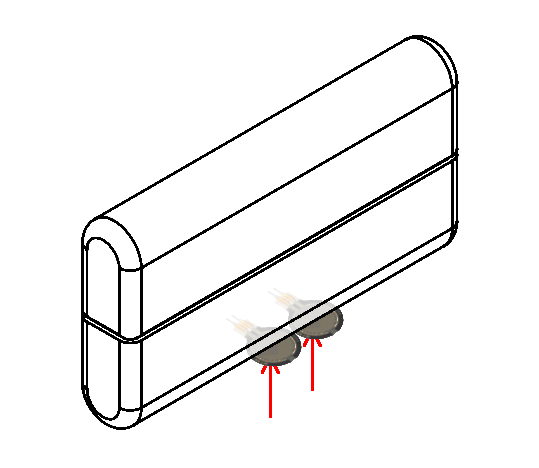
\includegraphics[width=\textwidth]{Figure/dummipalmside.png}
    \caption{Sensorized palm with FSRs}
    \label{fig:dummifsr}
  \end{minipage}
  %\caption{FSR sensors position on sensorized palm}
\end{figure}

Force is exchanged during a handshake only after the reference position has reach the first contact point $q_0$, therefore for values of $q < q_0$ no force will be exchanged in the handshake. %The constraints on $q$ introduced in \ref{sec:softhand} are valid through all this work since are hardware related.
The \textit{sensorized palm} is used in order to seek the force behaviour of the FSR sensors for values of the reference position $q > q_0$. 
It can be seen that once the hand makes contact with an object at position $q_a = q_0$, if it can be modelled as a rigid body, the actual hand configuration cannot change. Increasing the reference position result in a relationship
% it is enough stiff with respect to the hand, actual hand configuration cannot change even if we increase the reference one, and there is a relationship, 
that can be approximated as linear, between the difference $q-q_0$ and the force that the hand is applying to the object, $F_R$, i.e. 
%The shells of the device are not deformable, due to the material used during the 3D printing. Increasing the reference position $q$ of the Pisa/IIT SoftHand squeezing the \textit{sensorized palm} showed a linear relationship between the difference $q-q_0$ and $F_r$, as	 
%\textcolor{magenta}{talk about why the spring relation is choosed}

\begin{equation}
F_{r}(q)=\left\{\begin{matrix}
k_{r}(q-q_0) & $ for $ &q-q_0 \geq 0 \\ 
0 & $ for $ & q-q_0 < 0
\end{matrix}\right.
\label{eq:genericForce}
\end{equation}\\

%
%$$
%F_{r} = 
%  \begin{cases} 
%    $Dynamic to find$ & q-q_0 \geq 0 \\
%    0 & q-q_{0} < 0
%  \end{cases}
%$$\\
If the linear coefficient $k_{r}$ and position $q_0$ were known, we therefore could use this relationship to estimate $F_{r}$ from $q$.  
Where $F_r$ is the force during the handshake applied by the robot, $q$ is the reference position sent to the device, $q0$ is the first contact point and $k_{r}$ is a constant parameter to seek.
%The experiment is executed with a participant applying different forces on the above mentioned device, and recording the output from the FSR sensors and from the load cell of the \textit{sensorized palm}.
%The plot in Fig. \ref{Fig:FSRcalibratedModel}, shows the data obtain from this experiment.
Taking $N=2$ as the number of FSR sensors installed on the Pisa/IIT SoftHand, $F_{fsr,i}$ as the measure of the generic $i-th$ sensor, grasping force is estimated as %\eqref{eq:sumofFSR}.

\begin{equation}
\hat{F}_{fsr} = \sum_{i=1}^{N} F_{fsr,i}
\label{eq:sumofFSR}
\end{equation}

Using the Matlab Curve Fitting toolbox, we fitted a cubic polynomial to the experimental data and obtained a relationship between the sum of the measure of the sensors $\hat{F}_{fsr}$ and the load cell force $F_{fsr}$. The relationship can be expressed as:
%A toolbox for data fitting from Matlab has been used in order to find the best fitting equation, that includes the origin, according to the Least Mean Square Error to the raw data, which analytically is:

\begin{equation}
F_{fsr} = 2.86 \cdot 10^{-9}\cdot \hat{F}_{fsr}^3 - 1.85 \cdot 10^{-5} \cdot \hat{F}_{fsr}^2 + 0.049 \cdot \hat{F}_{fsr} 
\label{eq:fsrdummyfit}
\end{equation}

%where $\hat{F}_{fsr}$ is the value taken as the sum of the FSRs sensors, in this experiment two FSRs has been used. 
Forcing the equation to include the origin is a natural choice to avoid an offset in the force estimation f.i. if the measure of the FSRs is close to zero then the value of $F_{fsr}$ must be close to zero.
The variable $F_{fsr}$ is estimated from the load cell, and is returning Newtons and best explain the FSRs values with respect to the values of the \textit{sensorized palm}.
%due to the previous assumption is it represents the human grasping force measured by the FSR.
% 
 
\begin{figure}[h]
\centering
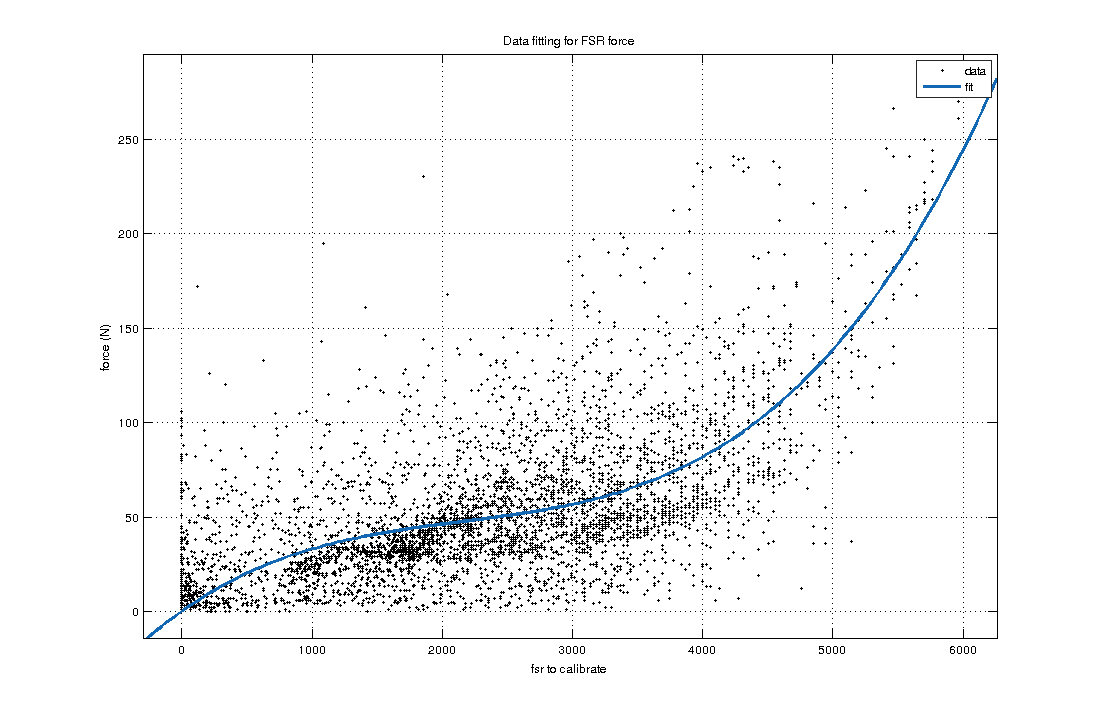
\includegraphics[width=0.9\textwidth]{Figure/fsrtodummy.png}
\caption{FSRs vs. Load Cell data}
\label{Fig:FSRcalibratedModel}
\end{figure}

Obviously, more advanced models can be fitted in order to have FSR sensors measurements with a higher precision, but for the specific task required in this work is considered sufficient the fitted equation in \eqref{eq:fsrdummyfit}. The handshake event is involving grasping forces in a limited range of forces, the fitted equation exists for $ \hat{F}_{fsr} \in \mathbb{R}$ but, physical limitation of the hardware (max absorbed current) are ensuring the upper bound of the force. Till this point nothing has been done on the Pisa/IIT SoftHand, the available information is that FSR sensors are returning values in Newton and have been calibrated according to a load cell sensor, therefore forces in the following chapters will be intended to be Newton scaled. 
%The data collected in this experiment contains several outliers from the fitted equation, this behaviour is due to the 
